\documentclass[a4paper, 12pt, finnish]{report} %dokumenttiluokka ja sille muutamia määrityksiä
\usepackage[utf8]{inputenc}
\usepackage{mathtools}
\usepackage{amsfonts}
\usepackage{eurosym}
%%\usepackage[toc,page]{appendix}
\usepackage{amsmath} %matematiikka kirjasto
\usepackage{graphicx} %kuvien liittämiseen kuten etusivun Aalto-logo
%\usepackage{pgfplots} %kuvaajien piirtämiseen, ota kommentointi pois mikäli haluat käyttää
\usepackage[finnish]{babel} %suomenkieli
\addto{\captionsfinnish}{\renewcommand{\bibname}{Lähteet}}
\usepackage{amsmath} %matematiikka kirjasto
\usepackage{graphicx} %kuvien liittämiseen kuten etusivun Aalto-logo
\usepackage{cite}
\usepackage[nottoc,numbib]{tocbibind}
\usepackage{titlesec}
\titleformat{\chapter}
{\Large\bfseries} % format
{}                % label
{0pt}             % sep
{\huge}           % before-code

\usepackage{hyperref}
\hypersetup{pdfpagemode=UseNone, pdfstartview=FitH, colorlinks=true,urlcolor=red,linkcolor=blue,citecolor=black,pdftitle={Kandityön suunnitelma},pdfauthor={Onni Lampi}}
%\usepackage{pgfplots} %kuvaajien piirtämiseen, ota kommentointi pois mikäli haluat käyttää

%\pagestyle{empty} %ei numeroita sivulle, mikäli niitä silti ilmestyy niin käytä komentoa \thispagestyle{empty} näillä sivuilla. Ei meinaa jostain syystä toimia report luokan kanssa
\setlength{\parindent}{0mm} %ei sisennystä uusiin kappaleisiin
\setlength{\emergencystretch}{15pt} %tekstin muokkaamiseen eli sallii välien venytyksen riveillä jotta näyttää paremmalta
\renewcommand{\bibname}{References}
\newcommand*{\findate}{\the\day.\the\month.\the\year} %uusi komento päivämäärän esittämiseen suomalaisittain
\newcommand*{\sijoitus}[2]{\mathop{\Big/}\limits_{\mspace{-19mu}#1}^{\mspace{19mu}#2}} % uusi komento jolla saadaan itgeraaliin suomalainen sijoitus viiva, käytetään \sijoitus{yläraja}{alaraja}, vaatii amsmath kirjaston
\renewcommand\thesection{\arabic{section}}
\usepackage{fancyhdr}
\usepackage{caption}
%\pagestyle{fancy}
%\fancyhf{}
%\rhead{Hekon logo}
%\lhead{Helsingin Kotkat ry - toimintakertomus 2015-2016}
\begin{document}

%\begin{center}
%
\includegraphics[width=50mm, scale=0.1]{heko.png}
%\end{center}
%\begin{center}
%	
\includegraphics[keepaspectratio=true,height=70mm]{heko.png}
%\end{center}
\chapter{Toimintakertomus 2016-2017}

\begin{figure}[htb]
	\begin{center}
		
\includegraphics[height=4cm]{heko.png}
	\end{center}
	%\caption{Kuvateksti, jossa on liitteen numerointi}
\end{figure}


\section{Yleistä lippukunnasta}
Helsingin Kotkat toteuttaa toiminnassaan Suomen Partiolaisten partio-ohjelmaa. Toiminta oli kuluneella kaudella aktiivista ja lippukunnan jäsenmäärä on vakaa.\\
\\Lippukunnassa toimi keväällä 2016 yksi tyttösudenpentulauma, kaksi poikasudenpentulaumaa, yksi tyttöseikkailijajoukkue, yksi poikatarpojajoukkue, yksi tyttötarpojaryhmä sekä yksi poikasamoajaryhmä.\\
\\Lisäksi lippukunnan johtajatehtävisä toimivat vaeltajat ja aikuiset ovat kokoontuneet toiminnansuunnittelun merkeissä.
\newpage
\section{Toiminta}
\subsection{Kokoukset}

\begin{figure}[htb]
	\begin{center}
		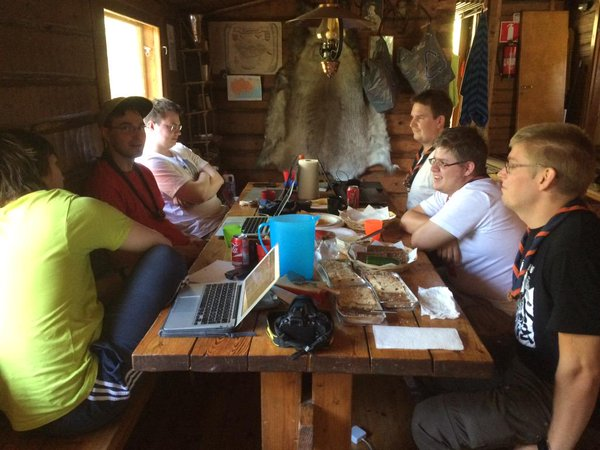
\includegraphics[height=7cm]{kokous.jpg}
	\end{center}
	\caption*{\textbf{Toiminnansuunnittelua lippukunnan kämpällä.}}
\end{figure}


Ryhmät koontuivat omiin tapaamisiinsa viikoittain ja johtajat pitivät omia kokouksiaan tarpeen mukaan, esimerkiksi retkien suunnittelua varten. Kokouksista ja niiden määrästä lista alla:\\
\begin{center}
	\begin{tabular}{ l l }
		Vuosikokous & 1 kpl\\
		Vaalikokous & 1 kpl\\
		Hallituksen kokous & 9 kpl\\
		Poikasamoajat & n kpl\\
		Tyttötarpojat & n kpl\\
		Tyttöseikkailijat & n kpl\\
		Poikaseikkailijat & n kpl\\
		Tyttösudenpennut & n kpl\\
		Poikasudenpennut & n kpl\\
						      & \\
		Yhteensä & x kpl\\
	\end{tabular}
\end{center}
Lisäksi vuoden mittaan on pidettu lukuisia muita pienempiä ja epävirallisia kokouksia, joissa on esimerkiksi suunniteltu toimintaa, retkiä tai kämppien kunnostusta.
\subsection{Leirit ja retket}
\subsubsection{Jouluretki}
\subsubsection{Kevätretki}
\subsubsection{SuSe-leiri}
\subsubsection{Ryhmien retket}
\subsection{Muu toiminta}
\subsubsection{Kisat}
\subsubsection{Kurssit ja koulutus}
\subsubsection{Varainhankinta}
\subsubsection{Muuta}
\section{Toimitilat}
\subsection{Kolo}
Lippukunnan pääasiallisena toimitilana, eli Kolona toimii Mellunmäki-Seuralta vuokrattu noin 50 neliömetrin kokoinen huone. Tilassa olevaa keittiötä alivuokrataan Hilkka Harjulle, joka käyttää tilaa päivisin.
\subsection{Varasto}
Lipukunnan retki- ja leirikalustoa säilytetään Sallatunturintie 1:ssä, jossa lippukunnalla on noin 30 neliömetrin kokoinen varastotila. 
\subsection{Willa}
Lippukunnan käytössä on Nuuksiossa yksityisellä luonnonsuojelualueella sijaitseva Willa-niminen kämppä. Kämpälle tehdään ryhmien toimesta retkiä muutaman kerran vuodessa. Kämpästä ei makseta vuokraa.
\subsection{Kyöpeli}
Lippukunnan pääasiallisena kämppänä toimii osoitteessa Ruuhijärventie 17 sijaitseva Kyöpeli. Kämppään kuuluu laajahko tontti. Kämppää käytetään lippukunnan omiin retkiin ulkopuolelle vuokrauksen lisäksi. Myös lippukunta maksaa omista retkistään vuokraa, jotta kämpän ylläpitoon saadaan riittävästi varoja.\\
\\Kämpän suhteen tehdään läheistä yhteistyötä Paakaupunkiseudun partiolaisten kanssa. Tämä näkyy siten, että lippukunnalla on 1/4-osa käyttöoikeus kaikkiin piirin tarjoamiin palveluihin. Näihin kuuluu sauna, vesikaivo ja jätehuolto.\\
\\Kyöpelillä vietetään joka vuosi talkoot, yleensä Helatorstaina. Tällä toimikaudella talkoissa tehtiin valtavat määrät puutöitä sekä uudet penkit nuotiopaikalle, lisäksi sisätiloissa tehtiin parannustöitä keittiöön.
\section{Jäsenet}
\section{Hallitus ja toimihenkilöt}
\begin{center}
	\begin{tabular}{ l l }
		\textbf{Hallitus} & \\
		Onni Lampi & lippukunnanjohtaja\\
		Hanna Tompuri & lippukunnanjohtajan apulainen\\
		Pyry Aaltonen & sihteeri, uudet jäsenet\\
		Eero Lilja & taloudenhoitaja, jäsenrekisterinhoitaja\\
		Pekka Holopainen & varasto- ja kolovastaava\\
		Heidi Ekblom & koulutusvastaava, viestintämestari\\
		Pauli Saarikoski & ohjelmavastaava\\
		Aapo Launiainen & kämppävastaava\\
					      & \\
		\textbf{Muut toimihenkilöt} & \\
		Kimmo Huurinainen & kirjanpitäjä\\
		Ari Söderqvist & toiminnantarkastaja\\
		Minna Söderqvist & varatoiminnantarkastaja\\
						& \\
		\textbf{Ryhmät ja niiden johtajat} & \\
		Poikasudenpennut & \\ 
	\end{tabular}
\end{center}


\section{Talous}
Lippukunta on säilynyt vakavaraisena läpi tilikauden. Lippukunta sai Urlus-säätiöltä 5000\euro{} avustusta Kyöpelin katon uusimiseen, tämä toteutetaan <joskus>. Lippukunta haki ja sai myös 1500\euro{} rahaa leirikalustonsa uusimiseen, tällä hankittiin uusi puolijoukkueteltta. Varoja koitetaan säästää tulevaisuutta varten, esimerkiksi suojaamaan nousevalta toimitilavuokralta.
\section{Taustayhteisöt}
\begin{figure}[htb]
	\begin{center}
		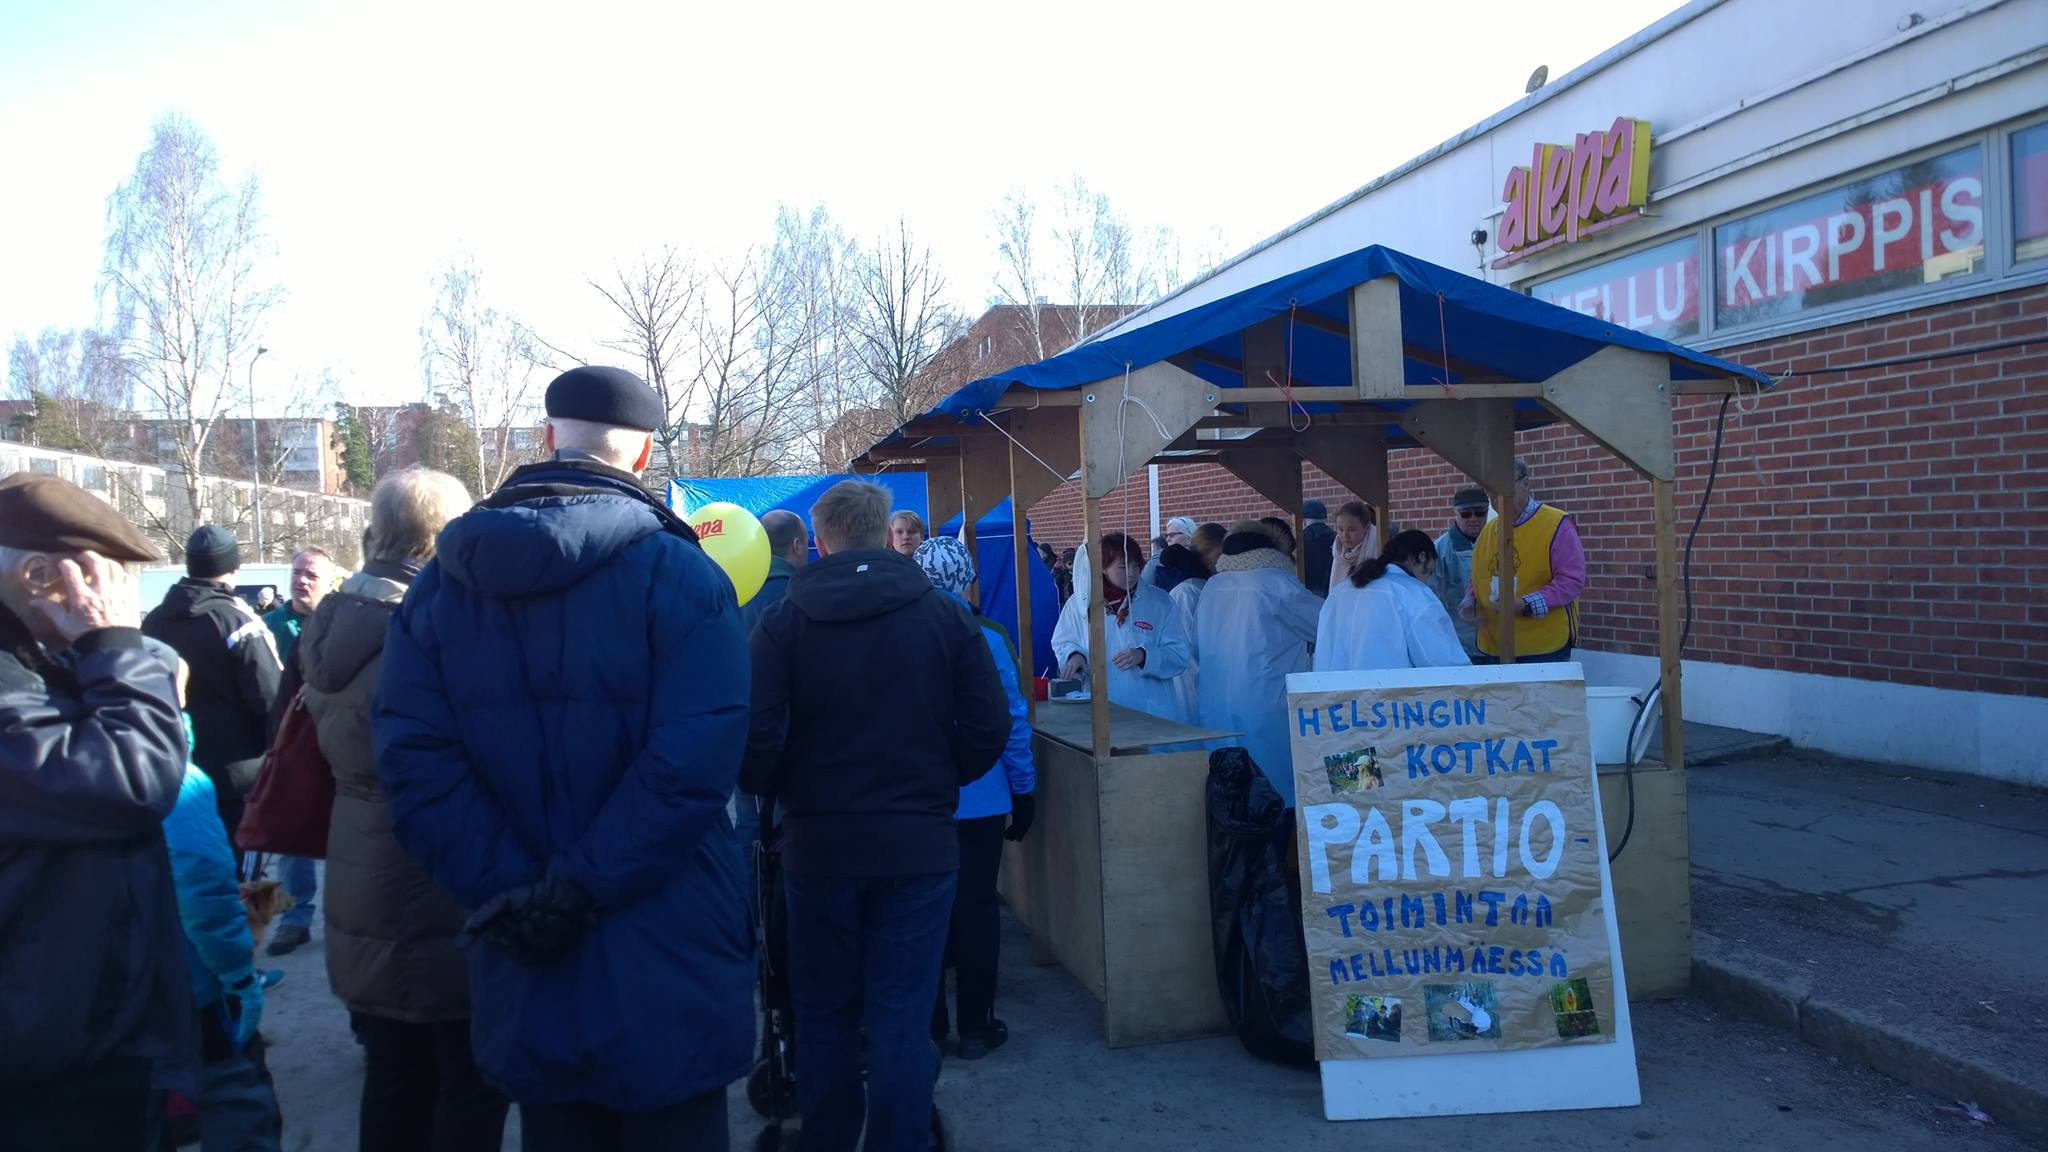
\includegraphics[height=7cm]{lettukestit.jpg}
	\end{center}
	\caption*{\textbf{Vohvelimyyntiä Mellunmäen Lionsien kevätriehassa.}}
\end{figure}

Taustayhteisöinä ovat tuttuun tapaan toimineet Mikaelin seurakunta, Mellunmäen Lions Club ja Partiolippukunta Helsingin Kotkat ry:n Venhempainyhdistys ry. Jokaiseen taustayhteisöön on oltu aktiivisesti yhteydessä ja heidän kanssaan on järjestetty tapahtumia.

\end{document}
